%!TEX root = ../../thesis.tex

Utilising the measurement methods used previously, a liquid that better replicates a biological impedance is sought.
This work is of benefit to engineers of medical implant devices.
Having the ability to formulate a solution that mimics the electrical conditions inside a living mammal reduces the resources required to test electronic implants.

It was previously mentioned that the developers of spinal cord stimulator implants used solutions of PBS having a one-tenth concentration as a test fluid for their implants.
This solution was the best substitute for an actual live spine that these engineers had.
Solutions of the \SI{0.1}{X} PBS are held in drums within the electronics laboratories for use whenever quick tests needed to be carried out.
Electrodes were submerged into these drums in order to recreate the electrical conditions inside a human spine.
This was not the only way to simulate the impedance conditions inside a person.
As presented in~\cref{sect:sheep_measurements}, anaesthetised sheep are also used.
A sheep's spine is smaller than a human's but is a good approximation in terms of geometry.
However, the resources involved with conducting a live sheep trial are high; requiring use of a hospital operating theatre, surgeon veterinarian, and equipment.
Engineers have no way of knowing how well those baths of saline represented a sheep's spine.
It was shown in \cref{sect:sheep_measurements} that the match between the two was weak.
With that knowledge, and the measurement techniques developed thus far, research into creating a solution that better matches sheep spine is carried out.
Strengthening that match would reduce the number of surgical operations the test engineers might need to conduct, saving resources and reducing time.

\section{Ingredients}

  To determine how certain additives affect the impedance of the interface, a range of ingredients are mixed and measured.
  Various mixtures were created using a heuristic approach until trends emerged which eliminated many of the ingredients.
  The following consumer grade ingredients were used for mixture testing and creation:
  \begin{itemize}
      \item Cellulose
      \item Citric acid
      \item Cornflour
      \item Gelatine
      \item Glycerol
      \item Isopropyl alcohol - 99.9\% pure
      \item Methylated spirits
      \item Potassium chloride - agricultural grade
      \item Sodium bicarbonate
      \item Sodium carbonate
      \item Sodium chloride - non-iodised
  \end{itemize}

  Those ingredients were chosen as they include alcohols, sugars, salts, acids, and inert fillers.
  The filling agents are expected to reduce the capacitive nature of the CPE by adding non participant species to the electrolyte.
  As the CPE's behaviour relies on being able to reorient, repel, and attract species in the liquid phase, those ingredients should reduce the overall effect.
  These ingredients are also easily obtainable in large quantities.


\section{Measurement}

  The focus when creating the solution is to match the CPE and series resistance of the sheep measurements to the newly-created solution.
  The measurement setup used to measure the CPE response and series resistance is mostly the same as was used for characterising PBS and the sheep's spinal cavity.
  This configuration differs only in the electrodes used on the array, necessary due to electrode two having its connection broken, and is shown in \cref{fig:creatingCSF_setup}.
  A \SI{10}{\kilo\ohm} resistor was used to measure the current driven between electrodes eight and three.
  It had a measured resistance of \SI{9.990}{\kilo\ohm}, as measured with a Fluke digital multimeter.

  \begin{figure}
      \centering
      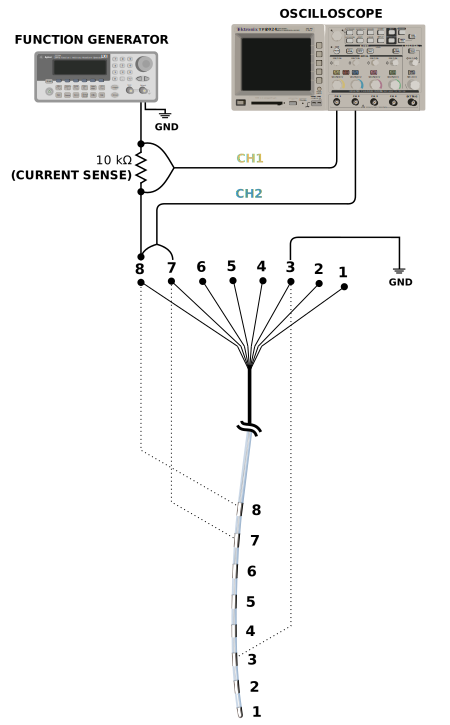
\includegraphics[scale=0.95]{content/pt2/graphics/CreatingCSF_setup}
      \caption{\label{fig:creatingCSF_setup}Diagram showing the measurement configuration used to measure the CPE response and resistivity of mixed solutions}
  \end{figure}

  Each measurement run begins at the upper end of the frequency spectrum and proceeds towards the low frequency endpoint.
  Starting with the higher frequencies offers a chance to confirm correct measurement set-up early in the measurement since they take less time to complete.
  A sample at the lowest frequency can take over a minute to acquire, where the higher frequencies take less than one second.
  The same frequencies were chosen that were used to measure the CPE's response in sheep's spinal cavity.
  Using those same frequencies makes comparison between the sheep data and the impedance of mixed solutions much easier.
  Measurements were fully automated via a Linux based computer running Python scripts.
  These scripts controlled the output settings of the waveform generator and acquired the resulting waveforms from the oscilloscope.
  The scripts had the ability to set the horizontal and vertical scales on the oscilloscope channels in order to ensure appropriate settings were used.
  \begin{figure}
      \centering
      
\includegraphics[width=\textwidth]{content/pt2/graphics/measurementFlowchart}
      \caption{\label{fig:creatingCSF_pythonFlowchart}Diagram showing the execution of the measurement script}
  \end{figure}
  The measurement procedure followed by the script is shown as a simplified flowchart in \cref{fig:creatingCSF_pythonFlowchart}.
  The programme steps through each of the required frequencies, making sure the target voltage is developed across electrodes seven and eight, before calculating the interface impedance.

  The target voltage across the interface is \SI{20}{\milli\volt}.
  This voltage was previously determined as a safe stimulus voltage in that it does not trigger Faradaic reactions at the electrode's surface and was used in for PBS measurements.
  Because the impedance of the interface changes with frequency it is necessary to alter the output amplitude to keep the voltage across electrodes seven and eight consistent.

  % Edit checkpoint 2015-09-19 14:49

\section{Results \& Discussion}

  \begin{figure}
    \centering
    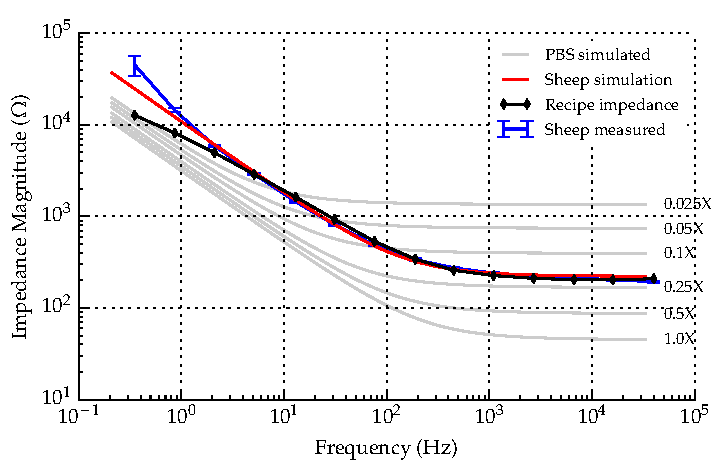
\includegraphics[width=\textwidth]{content/pt2/graphics/run14_175ml-distilledWater_250g-cornflour_1g9-salt_ZVsF_graph_mag}
    \caption{\label{fig:recipe_cornflour_salt_mag}Graph showing impedance magnitude versus frequency (log-log) for \SI{250}{\gram} cornflour mixed with \SI{175}{\milli\litre} distilled water and \SI{1.9}{\gram} table-salt.}
  \end{figure}

  \begin{figure}
    \centering
    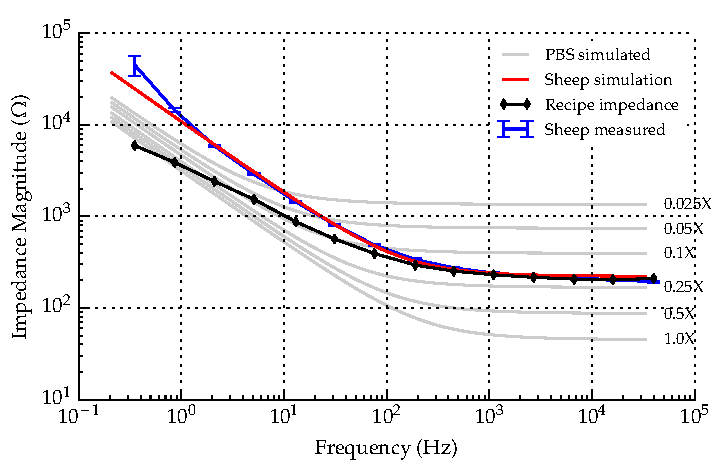
\includegraphics[width=\textwidth]{content/pt2/graphics/run14_180ml-distilledWater_250g-cornflour_1g9-salt_ZVsF_graph_mag}
    \caption{\label{fig:recipe_cornflour_salt_extraWater_mag}Graph showing impedance magnitude versus frequency (log-log) for \SI{250}{\gram} cornflour mixed with \SI{180}{\milli\litre} distilled water and \SI{1.9}{\gram} table-salt.}
  \end{figure}

  Not surprisingly, the salt had the greatest influence on the response per gram added.
  The other non-inert ingredients had much the same effect but required larger quantities to achieve the same effect.
  This suggests that the primary contribution those ingredients offered was increasing the overall conductivity.
  The salt was capable of bringing the broad-band response in line with each of the PBS traces, which were themselves salt based solutions.
  The real question was whether any of the ingredients would be capable of moving the CPE's slope independently of the solution's conductivity.
  A solution of 0.25X PBS roughly matches the bulk conductivity of sheep spine, however the sheep's spine offered a much higher impedance at low frequencies -- where the CPE dominates.
  What was needed was a way to increase the impedance offered by the CPE without affecting the bulk conductivity of the solution.

  One popular and fun use of cornflour is creating a non-Newtonian fluid by mixing it with water.
  It behaves like a classical fluid until pressure is applied to it, then it temporarily solidifies around the point of pressure.
  There is a critical point when creating the mixture when adding additional water quickly turns it from a dry mix to wet volume, i.e. the consistency becomes highly sensitive to relatively small quantities water being added.
  \Cref{fig:recipe_cornflour_salt_mag} shows the measured CPE response of a mixture of \SI{250}{\gram} cornflour, \SI{1.9}{\gram} salt, and \SI{175}{\milli\litre} of water, at the point when the mixture transitions from having a dry base to a wet one.
  This particular solution manages to match the impedance response to sheep better than any saline solution.
  What is interesting is what adding another \SI{5}{\milli\litre} of water did to the impedance response, shown in \cref{fig:recipe_cornflour_salt_extraWater_mag}.
  Adding cornflour to the saline solution made negligible difference to the response until close to the point when the water becomes saturated with cornflour; corresponding to that critical mixing point mentioned earlier.
  Comparing \cref{fig:recipe_cornflour_salt_mag} to \cref{fig:recipe_cornflour_salt_extraWater_mag}, the series resistance has stayed the same but the CPE slope has changed.
  No other ingredients tried changed the slope of the CPE's response and it appears as though the critical point of mixing the cornflour and water is having a large impact on that change.

  The drop in impedance at low frequencies may be a result of a lack of buffering agent in the saline solution.
  This drop is also seen in measurements of straight unbuffered saline solutions, indicating that it is not the addition of cornflour that is causing the drop.
  Adding a buffering agent to the cornflour and saline mixture would most likely remove that impedance drop.
  It may also be possible to create an increase in impedance at low frequency by increasing the capacity of the buffering agent.

  \begin{figure}
      \centering
      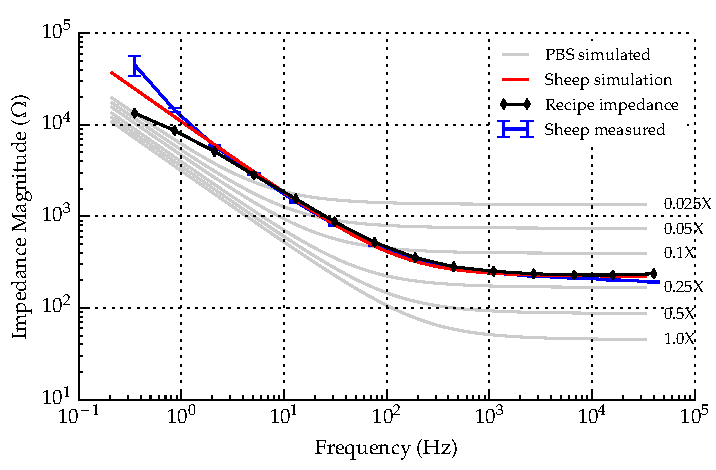
\includegraphics[width=\textwidth]{content/pt2/graphics/run12_190ml-distilledWater_190g-cornflour_0g858-salt_ZVsF_graph_mag}
      \caption{\label{fig:recipe_cornflour_salt_extraWater_mag_improved}Graph of measured impedance magnitude versus frequency (log-log) for \SI{190}{\gram} cornflour mixed with \SI{190}{\milli\litre} distilled water and \SI{0.858}{\gram} table-salt.}
  \end{figure}

  \begin{figure}
      \centering
      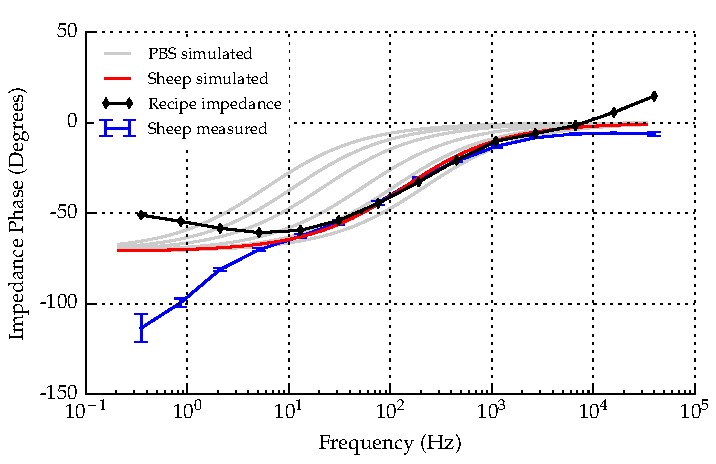
\includegraphics[width=\textwidth]{content/pt2/graphics/run12_190ml-distilledWater_190g-cornflour_0g858-salt_ZVsF_graph_phase}
      \caption{\label{fig:recipe_cornflour_salt_extraWater_phase_improved}Graph of impedance phase versus frequency (log-log) for \SI{190}{\gram} cornflour mixed with \SI{190}{\milli\litre} distilled water and \SI{0.858}{\gram} table-salt.}
  \end{figure}

  Finally, \cref{fig:recipe_cornflour_salt_extraWater_mag_improved,fig:recipe_cornflour_salt_extraWater_phase_improved} show both the magnitude and phase response of the closest match, as determined by a least squares error method.
  Again, the lack of buffering agent in these mixtures is expected to be responsible for the low frequency deviation from the measured response in sheep's spine.
  The ingredients that were used to create the final solution are summarised in \cref{tab:pt2-sheep-recipe}.
  These results are promising and no doubt will be of use not only to implant designers but to anyone trying to recreate the electrical impedance of biological fluids.

  \begin{table}
    \centering
    \begin{tabular}{r | r | c}
      Ingredient & Quantity & Unit \\
      \hline
      Cornflour & 190 & g \\
      Distilled water & 190  & ml  \\
      Salt  & 858 & mg  \\
    \end{tabular}
    \caption{\label{tab:pt2-sheep-recipe}Ingredients used to create the mixture that matches both the CPE's response and the interface series resistance.}
  \end{table}

  % Edit checkpoint 2015-09-20 20:53